% \begin{savequote}[8cm]
% Alles Gescheite ist schon gedacht worden.\\
% Man muss nur versuchen, es noch einmal zu denken.

% All intelligent thoughts have already been thought;\\
% what is necessary is only to try to think them again.
%   \qauthor{--- Johann Wolfgang von Goethe \cite{von_goethe_wilhelm_1829}}
% \end{savequote}

\chapter{\label{ch:2-background}Background}

    \minitoc

    \todo{Introduce that going to introduce notation and give the building blocks this thesis builds off}

    \todo{comment about notation like charlies, $\one$ for example}







    


\section{Markov Decision Processes}
\label{sec:2-1-mdps}

    \todo{chatgpt the intro stuff}

    In this section \textit{Markov Decision Processes} (MDPs) are introduced, along with related defintions of \textit{policies} and \textit{trajectories}. MDPs give a mathematical framework for problems concerning sequential decision making under uncertainty, and in this thesis will be the framework used to model the environment that agents act in. An MDP contains, among other things, a set of states and actions. States are sampled according to a transition distribution which depends on the current state and current action being taken (the Markov assumption). Any time an action is taken from a state the agent recieves an instantaneous reward, according to a reward function that depends on the state and action taken.

    This thesis is concerned with discrete, finite, fully-observable and finite-horizon Markov Decision Processes, meaning that the state and action spaces are discrete and finite, and any \textit{trajectories} (sequences of states, actions and rewards) are of a finite length. \todo{at points we may allude to some designs and ideas that can generalise to more general forms of markov decision processes, but it is not the main focus here.}

    \begin{defn}
        \label{def:mdp}
        A \textnormal{Markov Decision Process} (MDP) is a tuple $\cl{M}=(\cl{S},s_0,\cl{A},R,p,H)$, where $\cl{S}$ is a set of states, $s_0\in\cl{S}$ is an initial state, $\cl{A}$ is a set of actions, $R(s,a)$ is a reward function $\cl{S}\times \cl{A}\rightarrow \bb{R}$, $p(s' | s,a)$ is a next state transition distribution $\cl{S} \times \cl{A} \times \cl{S} \rightarrow [0,1]$ and $H\in\bb{N}$ is a finite-horizon time bound. 
    \end{defn}

    Notationally, it is convenient to define the set of successor states, that is the set of states that could be reached after taking an action from the current state of the MDP:
    \begin{defn}
        \label{def:succ}
        The set of \textnormal{successor states} $\suc{s}{a}$ of a state-action pair $(s,a)$, with respect to an MDP, is defined as: 
        \begin{align}
            \suc{s}{a}:=\{s'\in\cl{S}|p(s'|s,a)>0\}. \label{eq:succ_def}
        \end{align}
        
        Additionally, let $s'\sim \suc{s}{a}$ be a shorthand for $s'\sim p(\cdot|s,a)$.
    \end{defn}

    To define a strategy that an agent will follow in an MDP, and agent defines a \textit{policy}. A policy maps each state in the state space to a probability distribution over the action space. To ``follow'' a policy, actions are sampled from the distribution. Often it is desirable to define deterministic policies, which always produce the same action when given the same state, and can be represented as \textit{one-hot} distributions. 

    \begin{defn}
        \label{def:policy}
        A \textnormal{(stochastic) policy} $\pi:\cl{S}\rightarrow (\cl{A} \rightarrow [0,1])$ is a mapping from states to a probability distributions over actions and $\pi(a|s)$ is the probability of sampling action $a$ at state $s$. The policy $\pi$ must satisfy the conditions: for all $s \in \cl{S}$ we have $\sum_{a\in\cl{A}} \pi(a|s) = 1$ and for all $a\in\cl{A}. \pi(a|s)\geq 0$ . 
        
        Additionally, a \textnormal{deterministic policy} is defined as a one-hot policy, that is, the policy $\pi$ is deterministic iff it can be written as $\pi(a|s)=\one[a=a']$ for some $a'\in\cl{A}$.

        Moreover, the following notations are used for policies:
        \begin{itemize}
            \item $a\sim\pi(\cdot|s)$ denotes sampling an action $a$ from the distribution $\pi(\cdot|s)$;
            \item $\pi(s)=a'$ is used as a shorthand to define the deterministic policy $\pi(a|s)=\one[a=a']$; 
            \item $\pi(s)$ is used as a shorthand for the action $a'\sim\pi(\cdot|s)$ in the case of a deterministic policy.
        \end{itemize}
    \end{defn}
    
    Given an MDP $\cl{M}$ and a policy $\pi$ it is then possible to sample a sequence of states, actions and rewards, known as a \textit{trajectory}. A trajectory \textit{simulates} one possible sequence that could occur if an agent follows policy $\pi$ in $\cl{M}$, and in Section \todo{ref} these simulations are used to incrementally build a search tree.
    
    \begin{defn}
        \label{def:trajectory}
        A \textnormal{trajectory} $\tau$, is a sequence of state, action and rewards, that is induced by a policy $\pi$ and MDP $\cl{M}$ pair. Let the trajectory be $\tau = (s_0, a_0, r_0, s_1, a_1, r_1, ..., s_{H-1}, a_{H-1}, r_{H-1}, s_H)$, where $a_t \sim \pi(\cdot|s_t)$, $r_t=R(s_t,a_t)$ and $s_{t+1} \sim \suc{s_t}{a_t}$. 
        
        The following notations will also be used for trajectories:
        \begin{itemize}
            \item $\tau\sim\pi$ denotes a trajectory that is sampled using the policy $\pi$, where the MDP $\cl{M}$ is implicit;
            \item $\tau_{i:j}$ denotes the \textnormal{truncated trajectory} $\tau_{i:j}:=(s_i, a_i, r_i, s_{i+1}, ..., s_{j-1}, a_{j-1}, r_{j-1}, s_j)$, between the timesteps $0\leq i < j \leq H$ inclusive;
            \item $\tau_{:j}:=\tau_{0:j}$ denotes a trajectory that is trunacted on only one end.
        \end{itemize}
    \end{defn}

    \todo{citations in this section? Puttman?}







\section{Reinforcement Learning}
\label{sec:2-2-rl}



    \begin{figure}
        \centering
\includegraphics[width=0.5\textwidth]{figures/todo.jpg} 
        \caption[todo]{\todo{add diagrams of typical agent interacting with environment diagram, AND something with agent acting with a simulator. ALSO, WRITE THE BIT FOR THE CAPTION FOR LIST OF FIGS}}
        \label{fig:rl_overview}
    \end{figure}

    \todo{chatgpt the intro stuff}

    This section serves as a brief introduction to fundamental concepts in Reinforcement Learning, and motivates . The field of Reinforcement Learning considers an agent that has to learn how to make decisions by interacting with its environment (Figure \ref{fig:rl_overview}). The agent can take actions in the environment, recieving in return \textit{observations} and \textit{rewards}, which can be used to update internal state and used to make further decisions, and the goal of the agent is to maximise the rewards that it recieves.

    Classically the agent is considered to interact with its environment directly \todo{cite sutton and barto?}, and thus must make a trade-off between exploring new strategies and exploiting learned strategies, commonly known as the \textit{exploration-exploitation trade-off}. If an agent were to try to only exploit, then it may not discover better strategies, and if an agent only explores, then it may miss out on the opportunity to exploit the best known strategy and obtain greater rewards.

    Also depicted in Figure \ref{fig:rl_overview} is a scenario where the agent is equiped with a simulator that it can use to plan and explore, and is either asked to recommend a strategy after a planning/learning phase, or is occassionally queried to recommend actions. This scenario more closely resembles how reinforcement learning is used in the modern era with greater amounts of compute power available, and interactions with the simulator occur at orders of magnitude quicker. Hence, in this scenario, the only significant real-world cost comes from following the recommendations output, to be used in the real-world environment. This changes the nature of the exploration-exploitation trade off, almost separating the two issues, where there is an emphasis on exploring during the planning phase, and the problem of providing good recommendations is concerned with pure exploitation. 

    In this thesis, the environment will always take the form of an MDP (Defintion \ref{def:mdp}), and observations will always be \textit{fully-observable}, meaning that the agent is provided with full access to the states of the MDP. \todo{comment about partially observable? and cite?}. Moreover, a lot of the work in this thesis concerns the simulation scenario from Figure \ref{fig:rl_overview}, and motivates our research questions around exploration: \exploreq.

    Following on from Section \ref{sec:2-1-mdps}, the remainder of this section defines \textit{value functions} and the objectives of reinforcement learning, covers \textit{Value Iteration}, a tabular dynamic programming approach to reinforcement learning, and finally Subsection \ref{sec:2-2-merl} covers \textit{Maximum Entropy Reinforcement Learning}.
    
    The value of a policy $\pi$ is the expected cumulative reward that will be obtained by following the policy:
    \begin{defn}
        \label{def:value}
        \label{def:q_value}
        The \textnormal{value} of a policy $\pi$ from state $s$ at time $t$ is:
        \begin{align}
            V^{\pi}(s;t) = \bb{E}_{\tau\sim\pi}\left[\sum_{i=t}^{H-1} r_t \Bigg| s_t=s \right]. \label{eq:value_fn_def}
        \end{align} 

        The \textnormal{Q-value} of a policy $\pi$, from state $s$, with action $a$, at time $t$ is:
        \begin{align}
            Q^{\pi}(s,a;t) = R(s,a) + \bb{E}_{s'\sim \suc{s}{a}} [V^{\pi}(s';t+1)]. \label{eq:q_value_fn_def}
        \end{align} 
    \end{defn}

    From the definition of the values functions the optimal value functions can be defined by taking the maximum value over all policies:
    \begin{defn}
        \label{def:optimal_value}
        \label{def:optimal_q_value}
        The \textnormal{Optimal (Q-)Value} of a state(-action pair) is defined as:
        \begin{align}
            V^*(s;t) &= \max_{\pi} V^{\pi}(s;t) \label{eq:opt_value_fn_def} \\
            Q^*(s,a;t) &= \max_{\pi} Q^{\pi}(s,a;t). \label{eq:opt_q_value_fn_def}
        \end{align}
    \end{defn}

    Value functions can also be used to define an objective function:
    \begin{defn}
        The \textnormal{(standard) reinforcement learning objective function} $J(\pi)$ is defined as:
        \begin{align}
            J(\pi) = V^{\pi}(s_0;0). \label{eq:rl_obj_fn_def}
        \end{align}

        The objective of (standard) reinforcement learning can then be stated as finding $\max_{\pi} J(\pi)$.
    \end{defn}

    \todo{all refs below I think can be Sutton and Barto, or [Bellman 1957] Bellman, R. 1957. Dynamic Programming. Princeton, NJ, USA: Princeton University Press, 1 edition.}

    It can be shown that the optimal (Q-)value functions satisfy the \textit{Bellman equations} \todo{refs} :
    \begin{align}
        V^*(s;t) &= \max_{a\in\cl{A}} Q^*(s,a;t), \label{eq:bellman_opt_v} \\
        Q^*(s,a;t) &= R(s,a) + \bb{E}_{s'\sim \suc{s}{a}} [V^*(s';t+1)]. \label{eq:bellman_opt_q}
    \end{align} 

    The Bellman equations admit a \textit{dynamic programming} approach which can be used to computer the optimal value functions, known as \textit{Value Iteration} \todo{ref}. In Value iteration, a table of value estimates $\hat{V}(s;t)$ are kept for each $s,t$. Given any initial estimate of the value function $\hat{V}^{0}$, the \textit{Bellman backup} operations are:
    \begin{align}
        \hat{V}^{k+1}(s;t) &= \max_{a\in\cl{A}} \hat{Q}^{k+1}(s,a;t), \label{eq:value_iter_v_backup} \\
        \hat{Q}^{k+1}(s,a;t) &= \bb{E}_{s'\sim \suc{s}{a}} [R(s,a) + \hat{V}^k(s';t+1)]. \label{eq:value_iter_q_backup}
    \end{align}

    In each iteration of Value Iteration, these values are computed for all $s\in\cl{S}$, $a\in\cl{A}$ and $t\in\{0,1,...,H\}$. The Bellman equations can be shown to be \textit{contraction operators} \todo{refs}, which can be used to show that $V^{k}\rightarrow V^*$ as $k\rightarrow \infty$, and when the state and action spaces are discrete, they will converge in a finite number of iterations. \todo{refs}

    The \textit{optimal policy} is the policy that maximises the objective function $J$, can be shown to be deterministic \todo{conditions, finite?} \todo{cite}:
    \begin{defn}
        \label{def:optimal_policy}
        The \textnormal{optimal (standard) policy} $\pi^*$ is the policy maximising the standard objective function:
        \begin{align}
            \pi^* = \argmax_\pi J(\pi) \label{eq:opt_policy_def}
        \end{align}
        or equivalently, the optimal standard policy can be found from the optimal Q-value function:
        \begin{align}
            \pi^*(s) = \argmax_a Q^*(s,a). \label{eq:opt_policy_from_opt_q_value}
        \end{align}
    \end{defn}





    \subsection{Maximum Entropy Reinforcement Learning}
    \label{sec:2-2-merl}

        In \textit{Maximum Entropy Reinforcement Learning}, the objective function is altered to include the addition of an entropy term, \todo{which is used to encourage the agent to explore} \todo{double check with max entropy paper their motivation for adding entropy and cite}. 
        
        Let $\cl{H}$ denote the (Shannon) entropy function \todo{cite}:
        \begin{align}
            \cl{H}(\pi(\cdot|s)) = \bb{E}_{a\sim\pi(\cdot|s)}[-\log \pi(a|s)] = \sum_{a\in\cl{A}} \pi(a|s) \log \pi(a|s). \label{eq:shannon_entropy_def}
        \end{align}

        In the maximum entropy objective, the relative weighting of entropy terms is included using a coefficient $\alpha$, called the \textit{temperature}. In the maximum entropy objective, analogues of the value functions can be defined, which are typically referred to as \textit{soft (Q-)values}, and similarly the maximum entropy objective is often referred to as the \textit{soft objective}.

        Soft values are defined as follows:
        \begin{defn}
            \label{def:sft_value}
            \label{def:sft_q_value}
            The \textnormal{soft value} of a policy $\pi$ from state $s$ at time $t$ is:
            \begin{align}
                V_{\sft}^{\pi}(s;t) = \bb{E}_{\tau\sim\pi}\left[\sum_{i=t}^{H-1} r_t + \alpha\cl{H}(\pi(\cdot|s_i)) \Bigg| s_t=s \right]. \label{eq:sft_value_fn_def}
            \end{align} 

            The \textnormal{soft Q-value} of a policy $\pi$, from state $s$, with action $a$, at time $t$ is:
            \begin{align}
                Q_{\sft}^{\pi}(s,a;t) = R(s,a) + \bb{E}_{s'\sim p(\cdot|s,a)} [V_{\sft}^{\pi}(s';t+1)]. \label{eq:sft_q_value_fn_def}
            \end{align} 
        \end{defn}

        Similarly, optimal soft (Q-)values can be defined by taking the maximum over policies again:
        \begin{defn}
            \label{def:optimal_sft_value}
            \label{def:optimal_sft_q_value}
            The \textnormal{Optimal soft (Q-)Value} of a state(-action pair) is defined as:
            \begin{align}
                V_{\sft}^*(s;t) &= \max_{\pi} V_{\sft}^{\pi}(s;t), \label{eq:opt_soft_value_fn_def} \\
                Q_{\sft}^*(s,a;t) &= \max_{\pi} Q_{\sft}^{\pi}(s,a;t). \label{eq:opt_soft_q_value_fn_def}
            \end{align}
        \end{defn}



        HERE HERE HERE




        In maximum entropy reinforcement learning, the objective is to find a policy with maximal soft value:
        \begin{defn}
            The \textnormal{maximum entropy (or soft) reinforcement learning objective function} $J_{\sft}(\pi)$ is defined as:
            \begin{align}
                J_{\sft}(\pi) = V_{\sft}^{\pi}(s_0;0).
            \end{align}

            The objective of maximum entropy (or soft) reinfrocement learning can then be stated as finding $\max_{\pi} J_{\sft}(\pi)$.
        \end{defn}



        Equations similar to the Bellman equations, aptly named the \textit{Soft Bellman equations} can be defined \todo{cite levine}, which differ to equations (\ref{eq:bellman_opt_v}) and (\ref{eq:bellman_opt_q}) by the replacement of the $\max$ operation with a \textit{softmax} or \textit{log-sum-exp} operation (which is why the maximum entropy analogues are referred to as the \textit{soft} versions of their standard reinforcement learning counterparts).

        Similarly to standard reinforcement learning, it can be shown \todo{refs} that the optimal soft (Q-)value functions satisfy the \textit{soft Bellman equations}:
        \begin{align}
            V_{\sft}^*(s;t) &= \alpha \log \sum_{a\in\cl{A}} \exp\left( Q_{\sft}^*(s,a;t) / alpha \right), \\
            Q_{\sft}^*(s,a;t) &= R(s,a) + \bb{E}_{s'\sim \suc{s}{a}} [V_{\sft}^*(s';t+1)].
        \end{align} 



        Again, similarly to standard reinforcement learning, we can define \textit{soft Bellman backups} that admit an analogous algorithm to value iteration:
        \begin{align}
            V_{\sft}^{k+1}(s;t) &= \alpha \log \sum_{a\in\cl{A}} \exp\left( Q_{\sft}^{k+1}(s,a;t) / alpha \right), \\
            Q_{\sft}^{k+1}(s,a;t) &= R(s,a) + \bb{E}_{s'\sim \suc{s}{a}} [V_{\sft}^k(s';t+1)].
        \end{align}

        Finally, given the optimal soft value and soft Q-value functions, the optimal soft policy is known \todo{cite}:
        \begin{align}
            \pi_{\sft}^*(a|s;t) = \exp\left(\left(Q_{\sft}^*(s,a;t) - V_{\sft}^*(s;t)\right) / \alpha \right).
        \end{align}

    \subsection{Remaining todos for this chapter after first draft}

        \todo{Add a comment similar to DENTS paper where we will drop the t in notation. Make it quite bold somehow}














\section{Multi-Armed Bandits}
\label{sec:2-2-mab}

    \todo{This section has the most work left, going to handle it last to get to mostly complete ch faster}

    \todo{Introduce tree search using multi-armed bandits?}
    \hide{
    \begin{itemize}
        \item Would like to think a bit about some of the bandits work that sample actions (from adversarial I think), because they were similar to boltzmann search but I hadn't seen details about those works when writing dents
        \item Also the gradient based MAB stuff in sutton and barto book? Looks relevant? Maybe consider that as update to DENTS paper? Either way, another idea for getting good Go results.
    \end{itemize}
    }
    \todo{list}
    \begin{itemize}
        \item $R(s,a)$ is a random variable in MAB literature, but we're assuming it's a fixed value in RL
        \item Multi-Armed Bandits routines algos
        \item Exploring Bandits routines and algos
        \item Contextual Bandits routines and algos
    \end{itemize}

    \todo{Some waffel intro about this being used for decision making under uncertainty, but doesnt encorporate the sequential part of it. However, necessary for foundations, because much of sequential work builds ontop of this work}

    \todo{Also say that this can be viewed as a single state MDP with $\cl{S}=\{\bot\}$ and $\cl{A}=\{1,...,K\}$}

    \todo{some more waffelly shit about MABs}

    In the $K$-armed bandit problem, an agent is tasked with iteratively selecting one of $K$ arms, originally introduced by \todo{author} \todo{cite MAB orig}. In each iteration, once an arm is selected, say $x\in\{1,...,K\}$, and a reward $y$ is returned according to an unknown probability distribution $f_x$. Let $n$ be the number of rounds of this game that are played, and let $\mu_i=\bb{E}[y|x=i]$ be the expected reward of pulling arm $i$. 
    
    When analysing an algorithmic strategy for Multi-Armed Bandits (MABs), a quantity known as \textit{regret} is commonly used, which compares the cumulative reward obtained, compared to the maximal reward that could be obtained with full knowledge of $\{f_i\}$.

    \todo{work out how to deal with the issue of not having policies defined yet. thinhk this needs to be moved to after ch2.1}

    \todo{some sentence}, the process of a MAB is as follows:
    \begin{itemize}
        \item for $m$ in $\{1,...,n\}$:
        \item agent selects arm $x^m$ according to policy $\pi$
        \item agent recieves reward $y^m \sim f_{x^i}$
    \end{itemize}

    \begin{defn}
        The \textnormal{(cumulative) regret} of the agent in the above process is defined as:
        \begin{align}
            \creg_{\mab}(\pi,n) = n\mu^* - \sum_{i=1}^n y^i,
        \end{align}
        where $\mu^* = max_i \mu_i$.
    \end{defn}

    To theoretically analyse algorithms for MAB problems, the quantity of expected regret, $\bb{E}[\creg_{\mab}]$ is considered. In \todo{cite} it is shown using information theory that there is a lower bound on the expected regret that an agent can achieve of $\Sigma(\log N)$, and in \todo{cite ucb} the Upper Confidence Bound (UCB) algorithm is introduced, achieving a matching upper bound of $O(\log N)$. 

    Let $N^m(j)$ be the number of times that arm $i$ has been pulled after $m$ rounds, $\bar{y}_i^m$ is the sample average of rewards recieved when pulling arm $i$: 
    \begin{align}
        \bar{y}_i^m=\frac{1}{m}\sum_{j=1}^m y^j \one[x^j=i].
    \end{align} 
    
    Then the arm selected by the UCB algorithm on the $m$th round is given by:
    \begin{align}
        \pi_{\ucb}(m) = \argmax_{j\in\{1,..,K\}} \bar{y}_j^m + b_{\ucb} \sqrt{\frac{\log(m)}{N(j)}} 
    \end{align}

    \todo{define $b_{\ucb}$}

    \todo{talk about explortaiton-exploitation trade off -- see Edwin thesis too because said it nicely}




    \subsection{Exploring Bandits}
    \label{sec:2-2-1-exploring-mab}

        In the pure exploration $K$-armed bandit problem \todo{cite},
        %https://link.springer.com/chapter/10.1007/978-3-642-04414-4_7#preview, 
        the game is changed slighly. The agent still gets to pull an arm each round, but after it recieves a reward each round it is given the opportunity to output a \textit{recommendation}. In exploring multi-armbed bandits (EMABs), the emphasis is now on the algorithm being able to provide the best recommendations possible, rather than trying to exploit pulling the best arm each round. In essence, this change seperates the needs to explore and exploit, the agent needs to explore with its arm pulls, and output an exploiting recommendation at the end of each round.

        \todo{some sentence}, the process of a EMAB is as follows:
        \begin{itemize}
            \item for $m$ in $\{1,...,n\}$:
            \item agent selects arm $x^m$ according to policy $\pi^m$
            \item agent recieves reward $y^m \sim f_{x^m}$
            \item agent outputs a recommendation policy $\psi^m$
        \end{itemize}

        Under this regime, the performance of an algorithm can be analysed by considering the quantity of \textit{simple regret} of the recommendation policy. The simple regret is the expected value of an \textit{instantaneous regret}, \todo{define instantaneous regret} which would come from following the recommendation policy.

        \begin{defn}
            The \textnormal{simple regret} of following the recommendation policy $\psi^m$ on the $m$th round is:
            \begin{align}
                \sreg_{\emab}(m) = \bb{E}_{i\sim\psi^m}[\mu^* - \mu_i].
            \end{align}
        \end{defn}

        \todo{talk about the bounds they show in their work}

        \todo{describe the algorithm which is pulling arms 1,2,...,K,1,2,...,K,1,..., and so on, and then recommending the arm that has the best empirical average}.



    
    \subsection{Contextual Bandits}
    \label{sec:2-2-2-contextual-mab}

        \todo{sleepy and rushed this section a bit}

        In the contextual $K$-armed bandit problem \todo{cite}, on each round the algorithm is given a context $w\in \cl{W}$, which the algorithm does not choose. If contextual multi-armed bandit problems (CMABs), the distribution that the rewards are drawn from now depend on $w$, written $f_{w,i}$ for context $w$ for arm $i$. 

        \todo{some more words around when this is useful and why, and define CMABs}

        \todo{some sentence}, the process of a MAB is as follows:
        \begin{itemize}
            \item for $m$ in $\{1,...,n\}$:
            \item agent recieves context $w^m$
            \item agent selects arm $x^m$ according to policy $\pi$
            \item agent recieves reward $y^m \sim f_{w^m,x^m}$
        \end{itemize}

        Similar to MABs and EMABs, the notion of regret is used to analyse CMABs. Specifically, \textit{contextual regret} is defined similarly to cumulative regret \todo{ref}, while taking into account the contexts drawn.

        \begin{defn}
            The \textnormal{(cumulative) contextual regret} of the agent in the above process is defined as:
            \begin{align}
                \ctxreg_{\cmab}(\pi,n) = \sum_{i=1}^n \mu_{w^i}^* - y^i,
            \end{align}
            where $\mu_{w}^* = \max_i \mu_{w,i}$.
        \end{defn}

        \todo{add definitions for $\mu_{w,i}$}

        \todo{Talk about contextual zooming precursor (need to read and add to litrev)}

        \todo{Write about contextual zooming, using CHMCTS paper, and use opportunity to add to litrev}



















\section{Trial-Based Heuristic Tree Search and Monte-Carlo Tree Search}
\label{sec:2-3-thts}

    \todo{list}
    \begin{itemize}
        \item Give high level overview of MCTS (why use it etc)
        \item Outline that I'll present this as here is THTS, and then here's the THTS routines for MCTS
    \end{itemize}

    \begin{figure}
        \label{fig:thts}
        \centering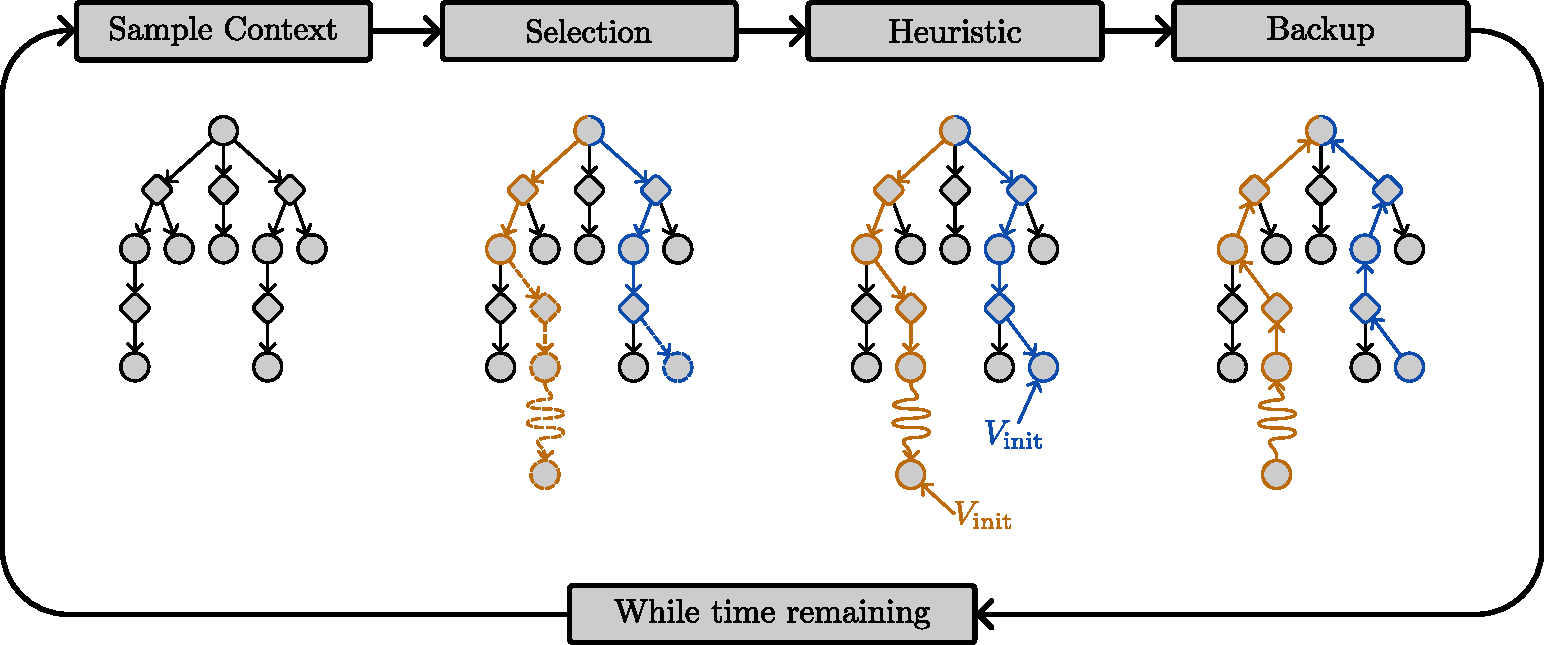
\includegraphics[width=0.9\textwidth]{figures/ch2/mcts_diagram_draft.pdf} 
        \caption[Overview of one trial of \thtspp.]{Overview of one trial of \thtspp, where orange shows an example when \mctsmode\ewe is True, and blue shows an example when \mctsmode\ewe is False. From left to right: first a context is sampled, which stores any necessary per-trial state (not depicted) and the search tree at the beginning of the trial is shown; second shows the selection phase, where dashed lines indicate any new nodes added; third shows that new leaf nodes are initialised using the $\Vinit$ heuristic function; and finally on the right, shows the backup phase, where the arrows directions are changed to show that information is being propogated back up the tree. \todo{fix the sligt noise in the dual blue and orange nodes}}
    \end{figure}

    \todo{double check the intro to 2.2, as wrote this a while ago}

    \todo{try to make sure specific about using thts vs mcts}

    In this section we introduce \thtspp\ewe \cite{thtspp}, which is an open-source, parallelised extension of the  Trial-based Heuristic Tree Search schema \cite{thts} (THTS). This schema is a generalisation of Monte Carlo Tree Search (MCTS), as presented in Section \ref{sec:2-2-2-mcts}. In \thtspp\ewe trees consist of \textit{decision nodes} and \textit{chance nodes}. Decision nodes output actions that can be taken by the agent, and chance nodes output \textit{outcomes} that may be random and may depend on the action taken. As such, each decision node has an associated \textit{state} and each chance node has an associated \textit{state-action pair}. In this work, we are considering fully-observable environments, but \thtspp\ewe can be generalised to consider \textit{partially-observable} environments. We give \thtspp\ewe implementations of the standard Upper Confidence Bound applied to Trees (UCT) algorithm and Maximum ENtropy Tree Search (MENTS) in Sections \ref{sec:2-2-2-mcts} and \ref{sec:2-2-3-ments} respectively.

    \todo{comments about how most MCTS algorithms are using a multi-armed bandit algorithm at each node}

    In MCTS we run trials, either for some fixed number of trials, or some timelimit, where each trial is split into four stages: 
        (1) selection, which samples states and actions for the trial, corresponding to a path down the tree;
        (2) expansion, which creates any new nodes in the tree; 
        (3) initialisation, which initialises values at any new leaf nodes in the tree;
        (4) backup, which updates values at all nodes visited on the trial.

    \todo{add MCTS figure here?}

    \begin{lstlisting}
def foo(bar):
        print("helloworld!")
    \end{lstlisting}

    \subsection{Trial Based Heuristic Tree Search}
    \label{sec:2-3-1-thts}
    
        \todo{list}
        \begin{itemize}
            \item{Copy DENTS MCTS section presentation, make a notation } $\texttt{node}(s_t)$ for the node at state $s_t$
            \item Present thts++
            \item Indicate what parts are new versus the original paper (context function, optionally running \mctsmode\ewe and mutli-threading)
            \hide{\item Small comment about multi-threading and two-phase locking used to avoid deadlock}
            \hide{\item TODO: probably not necessary to say - but thought of nice/concise way of explaining it (a node can lock children, not parent, if need info from parent, then it has to put a thread safe copy in the context)}
            \item Define terms precisely and consistently, for example \mctsmode\ewe (say that notation and terminology varies widely in literature, e.g. does uct run in mcts mode or not?)
            \item Mention that $\Vinit$ can be implemented as $V_\theta$ to be used with deep RL methods
            \hide{\item \todo{Find the best place to talk about deep RL? Maybe in the RL section?}}
        \end{itemize}

        \todo{this section relly really needs diagrams}

        \todo{add psuedo code}

        \todo{need to talk about contexts here again...}

        In this section we will present \thtspp schema, which is \todo{adaptation?} of the Trial-Based Heuristic Tree Search (THTS) schema \todo{cite}. After we have presented \thtspp, we will use the schema to define tree search algorithms that are relevant in this thesis, namely Upper Confidence Bound Applied to Trees (UCT) \todo{cite} in subsection \todo{ref} and Maximum ENtropy Tree Search (MENTS) in subsection \todo{Ref}. Finally we will briefly point out the differences between \thtspp and the original THTS schema in subsection \todo{ref}.

        \todo{this is already a subsection, so update above}

        In \thtspp\ewe a search tree $\cl{T}$ is built using Monte Carlo trials. Each trial is split into two phases: the \textit{selection phase} where a trajectory is sampled using a \textit{search policy}; and the \textit{backup phase} where value estimates stored in the tree structure are updated. In \thtspp\ewe the selection phase encumpasses the expansion and initialisation phases \todo{of the common presentation of MCTS}, where new nodes are added to the tree and the values of any new leaf node is initialised. 

        \todo{be more presise about trajectory vs trial, and update for sect 2.1}.

        To simplify notation in the presentation of \thtspp\ewe we will assume that states and state-action pairs have a one to one correspondance with nodes in the search tree $\cl{T}$. This assumption is purely to simplify notation for a clean presentation, and any results discussed in this thesis generalise to when this assumption does not hold. Given this assumption, we can state that the search tree is a subset of the state and state-action spaces, that is $\cl{T}\subseteq \cl{S} \cup \cl{S} \times \cl{A}$. \todo{rephrase last sentance for defn}

        \begin{defn}
            A \textnormal{search tree} $\cl{T}$ is a subset of the state and state-action spaces, that is $\cl{T}\subseteq \cl{S} \cup \cl{S} \times \cl{A}$, where for each $s\in\cl{T}$, there exists some trajectory $\tau_{:h}$ such that $s_h = s$, each $s'\in\tau_{:h}$ is also in the tree $s'\in\cl{T}$ and each $s',a'\in\tau{:h}$ is also in the tree $(s',a')\in\cl{T}$.
        \end{defn}

        \todo{clean above defn up}

        \todo{probably want to explicitly define what it means for s or s,a to be in a trajectory}

        \todo{words about decision and chance nodeS?}

        \begin{defn}
            A \textnormal{decision node} refers to any state that is in the search tree: $s\in\cl{T}$. A \textnormal{chance node} refers to any state-action pair that is in the search tree: $(s,a)\in\cl{T}$. And a \textnormal{node} is used to refer to any decision or chance node in the tree. When it is not clear from context if an $s$ or $(s,a)$ refers to a state(-action pair), the notation $\node(s)$ and $\node(s,a)$ will be used. \todo{fix node notation here}
        \end{defn}

        Additionally, each decision and chance node will generally store value estimates that are algorithm dependent. To specify this we will use $\node(s).V$ to denote the set of values stored at node $\node(s)$, and $\node(s,a).Q$ for the set of value stored at node $\node(s,a)$. \todo{make this a defn?}

        \todo{define N(s) and N(s,a)}

        The initial search tree consists of a single root node that corresponds to the initial state of the MDP: $\cl{T}^0=\{s_0\}$. And let $\cl{T}^k$ denote the search tree of \thtspp\ewe after $k$ trials have been run.

        To specify an algorithm in the \thtspp\ewe schema, the following need to be provided:
        \begin{description}
            \item[Search policy:]
                A distribution  $\pi^{k}$ for the $(k+1)$th trial, which can use values in the current search tree $\cl{T}^{k}$;
            \item[Heuristic function:]
                A function $\Vinit$ used as a heuristic to initialise values for new desicion nodes added to the tree;
            \item[Backup function:]
                Two functions $\cl{B}_V$ and $\cl{B}_Q$ which updates values; \todo{Clewan this up, and word better pls}
            \item[MCTS mode:]
                A boolean \mctsmode specifying if \thtspp\ewe should operate in MCTS mode.
        \end{description}

        \todo{actually define the above things properly somewhere}

        The $k+1$th trial of the \thtspp\ewe schema operates as follows: \todo{this is probably better written as psuedocode...}
        \begin{enumerate}
            \item sample a trajectory $\tau_{:h}$ using the search policy $\pi^{k}$;
            \begin{itemize}
                \item If \mctsmode\ewe is False, then $h=H$;
                \item If \mctsmode\ewe is True, then $h$ is such that $s_{h-1}\in\cl{T}^k$ and $s_h\not\in\cl{T}^k$, or $h=H$.
            \end{itemize}
            \item Any new nodes nodes that need to be added from this trajectory are added to the tree, $\cl{T}^{k+1} = \cl{T}^k \cup \tau_{:h}$;
            \item If $s_h\not\in\cl{T}^k$ then $\node(s_h).V$ is initialised using $\Vinit$;
            \item The backup functions are used to update values in the tree:
            \begin{itemize}
                \item For $i={h-1,h-2,...,1,0}$:
                \begin{itemize}
                    \item $\node(s_i,a_i).Q \leftarrow \cl{B}_Q(\{\node(s').V | s'\in\node(s_i,a_i).\children\})$
                    \item $\node(s_i).V \leftarrow \cl{B}_V(\{\node(s_i,a').Q | a'\in\node(s_i).\children\})$
                \end{itemize}
            \end{itemize}
        \end{enumerate}

        \todo{converting the above into some psuedocode. Should probably define children as a property of nodes. Should also just state that } $\node(s_i,a_i).Q$ \todo{and so on are just scalar values for now. We can make them vectors when needed later}. \todo{also make sure define } $N(s)$ and $N(s,a)$
        \begin{lstlisting}[caption={Psuedocode for running a trial in \thtspp}, label={lst:thts_trial}]
def run_trial(search_policy: $\pi$, heuristic_fn: $\Vinit$):
    $\tau_{:h}$ = sample_trajectory($pi$)
    if $s_h\not\in\cl{T}$:
        initialise_values($s_h$, $\Vinit$)
    for i in $\{$h-1,h-2,...,1,0$\}$:
        backup_q($s_i$,$a_i$)
        backup_v($s_i$)

def sample_trajectory(search_policy: $\pi$):
    pass

def initialise_values($s_h$, $\Vinit$):
    pass 

def backup_q($s_i$, $a_i$):
    pass
    
def backup_v($s_i$):
    pass
        \end{lstlisting}
        % TODO: make a figure env for code

        \todo{define } $\node(s_i).\children$ and $\node(s_i,a_i).\children$.

        \todo{Check how thts deals with using value estimates when children dont exist. There should be some form of using heuristic. Maybe this needs to be added to THTSpp todo list}

        \todo{Basically want to say that the 0th version of any estimate is filled using the Vinit and Qinit functions where necessary. So for example if a chance node doesnt exist yet then use Qinit.}

        \todo{should also be more clear that bottom node is initialised } $s_h$ \todo{using Vinit in the backup phase, and the rest use the backups}

        \todo{make sure neurips paper writing integrated (commented out, and below this comment in the .tex) - read the actual pdf for thesis and neurips papers and compare cover same info?}

        \todo{talk about the differences between thtspp and thts}
% MCTS methods build a search tree $\cl{T}$ using Monte-Carlo trials. Each trial is split into two phases: starting from the root node, actions are chosen according to a \textit{search policy} and states sampled from the transition distribution until the first state not in $\cl{T}$ is reached. A new node is added to $\cl{T}$ and its value is initialised using some function $V^{\text{init}}$, often using a \textit{rollout policy} to select actions until the time horizon $H$ is reached. In the second phase, the return for the trial is back-propagated up (or `backed up') the tree to update the values of nodes in $\cl{T}$. For a reader unfamiliar with MCTS, we refer to \cite{browne2012survey} for a review of the MCTS literature, as many variants of MCTS exist and may vary from our description. 

%         Two critical choices in designing an MCTS algorithm are the search policy (which needs to balance exploration and exploitation) and the backups (how values are updated). MCTS algorithms are often designed to achieve \textit{consistency} (i.e. convergence to the optimal action in the limit), which implies that running more trials will increase the probability that the optimal action is recommended.
%         % which gives the desirable property that running more trials should improve the policy.
        
%         To simplify notation we assume that each node in the search tree corresponds to a unique state, so we may represent nodes using states. Our algorithms and results do not make use of this assumption, and generalise to when this assumption does not hold.


    

    
    \subsection{Upper Confidence Bounds Applied to Trees (UCT)}
    \label{sec:2-3-2-uct}
    
        \todo{list}
        \begin{itemize}
            \item Define UCT here
        \end{itemize}

        \todo{I'm feeling ill writing this section, so just going to word vomit this shit out and make it sound not shit later}

        \todo{add Quct commands like Qments}

        Upper Confidence Bounds Applied to Trees (UCT) \todo{cite} is a commonly used tree search algorithm, which is based on the Upper Confidence Bounds (UCB) \todo{cite both papers} algorithm for Multi-Armed Bandit problems \todo{cite original MAB and a review}.

        In the literature, UCT and MCTS are often used synonomously, however this leaves some of the specifics of the algorithms used as ambiguous. In this thesis, we will present UCT as it was originally presented in \todo{cite}. And in subsection \todo{ref} we will specify the variant of UCT which is commonly referred to as MCTS.

        UCT can be defined using the THTS schema outlined in section \todo{ref} as follows:

        Firstly, UCT as originally presented is run with \mctsmode set to False. As such, all sampled trajectories are sampled until timestep $H$, the finite horizon of the MDP. 

        At each node a the sampled averages $\bar{V}_{\uct}$ or $\bar{Q}_{\uct}$ for value estimates.

        The search policy that UCT follows is:
        \begin{align}
            \pi_{\uct}(s) = \argmax_{a\in\cl{A}} Q_{\uct}(s,a) + b_{\uct} \sqrt{\frac{\log(N(s))}{N(s,a)}} 
        \end{align}
        \todo{add labels for equations}

        In \todo{ref above eqn}, when $N(s,a)=0$ there is a division by zero, which is taken as $\inf$, and ties are broken randomly, which effectively implements the ``every arm is initialised by pulling it once'' \todo{actually quote the paper, and cite UCT paper}. \todo{define the bias param}

        After sampling a trajectory $\tau_{:H}\sim\pi_{\uct}$ are updated as follows:
        \begin{align}
            \bar{Q}_{\uct}(s_t,a_t) &\leftarrow 
                \frac{1}{N(s,a)} \left( (N(s,a)-1) \bar{Q}_{\uct}(s_t,a_t) 
                    + \sum_{i=t}^{H-1} R(s_i,a_i) \right) \\
            \bar{V}_{\uct}(s_t) &\leftarrow 
                \frac{1}{N(s,a)} \left( (N(s,a)-1) \bar{V}_{\uct}(s_t,a_t) 
                    + \sum_{i=t}^{H-1} R(s_i,a_i) \right) 
        \end{align}  
        \todo{add labels for equations}

        \todo{Some note about the V values not actually being used in the algorithm}

        \todo{some comment about it can be implemented as backups (copy equations from THTS), but typically implemented as above. OR, just define backup functions to take the trajectory too}

        Because UCT is planning in a finite horizon MDP, the heuristic function will only be called on states that are at the time horizon H. As such, for UCT we can set $\Vinit(s) = 0$.

        \todo{add polynomial UCT here? and or prioritised UCT from alpha go here?}

        \todo{make sure neurips paper writing integrated in UCT and MCTS section (commented out, and below this comment in the .tex) - read the actual pdf for thesis and neurips papers and compare cover same info?}

        \todo{add stuff about regret here}
%         \paragraph{UCT} 
%             UCT~\cite{kocsis2006uct} applies the upper confidence bound (UCB) in its search policy to balance exploration and exploitation. The $n$th trial of UCT operates as follows: let $\cl{T}$ be the current search tree and let $\tau=(s_0,a_0,...,a_{h-1},s_{h})$ denote the trajectory of the $n$th trial, where $s_h\not\in\cl{T}$ or $h=H$. At each node $s_t$ the UCT search policy $\pi_{\text{UCT}}$ will select a random action that has not previously been selected, otherwise, it will select the action with maximum UCB value:
%             %
% %            \begin{align}
% %                \pi_{\textnormal{UCT}}^n(s_t) &= \max_{a\in\cl{A}} \text{UCB}^n(s_t,a), \\
% %                \text{UCB}^n(s_t, a) &= \bar{Q}^{N(s_t,a)}(s_t, a)+c \sqrt{\frac{\log N(s_t)}{N(s_t, a)}},
% %            \end{align}
%             \begin{align}
%                 \pi_{\textnormal{UCT}}(s) &= \max_{a\in\cl{A}} \bar{Q}(s, a)+c \sqrt{\frac{\log N(s)}{N(s, a)}}, \label{eq:uct_distr}
%             \end{align}
%             %
%             \noindent where, $\bar{Q}(s,a)$ is the current empirical Q-value estimate, $N(s)$ (and $N(s,a)$) is how many times $s$ has been visited (and action~$a$ selected) and $c$ is an exploration parameter. Then, $s_h$ is added to the tree: $\cl{T}\leftarrow \{s_h\}\cup\cl{T}$. The backup consists of updating empirical estimates for $t=h-1,...,0$:
%             %
%             \begin{align}
%                 \bar{Q}(s_t, a_t) &\leftarrow \bar{Q}(s_t, a_t) + \frac{\bar{R}(t) - \bar{Q}(s_t, a_t)}{N(s_t, a_t) + 1}, \label{eq:uct_qbar}
%             \end{align}
%             %
%             \noindent where $\bar{R}(t) = V^{\text{init}}(s_h) + \sum_{i=t}^{h-1} R(s_i,a_i)$, and $V^{\text{init}}(s_h)=\sum_{i=h}^{H} R(s_i,a_i)$ if using a rollout policy.



    
    \subsection{Monte-Carlo Tree Search}
    \label{sec:2-3-3-mcts}

        \todo{list}
        \begin{itemize}
            \item Give overview of MCTS
            \item Give UCT in terms of THTS schema 
            \item Define terms precisely and consistently in terms of THTS functions, maybe \mctsmode\ewe should go here
            \item Define the value initialisation of THTS using a rollout policy for MCTS
            \item Talk about the things that are ambiguous from literature (e.g. people will just say UCT, which originally presented doesn't run in \mctsmode, but often assumed it does)
            \item Should talk about multi-armed bandits here?
        \end{itemize}

        \todo{I'm feeling ill writing this section, so just going to word vomit this shit out and make it sound not shit later}


        \todo{add Qmcts commands like Qments}

        In this thesis we will refer to any algorithm that only adds one decision node to the search tree on each trial as an MCTS algorithm. That is any THTS algorithm with \mctsmode set to True is an MCTS algorithm. 

        In this section we will present what is commonly referred to as MCTS in the literature, where the heuristic function is either in the form of a \textit{rollout}, using a \textit{rollout policy} \todo{cite papers that do this, including some that just call it UCT}, or use a function $V_\theta$ that aims to approximate the true optimal value function $V^*$ from Equation \todo{ref} \todo{cite papers that do this}.

        These algorithms follow the same 

        These algorithms use the similar value functions to UCT, $\bar{V}_{\mcts}$ or $\bar{Q}_{\mcts}$. 

        The search policy corresponds to the UCT search policy, using the new $\bar{Q}_{\mcts}$ values:
        \begin{align}
            \pi_{\mcts}(s) = \argmax_{a\in\cl{A}} Q_{\mcts}(s,a) + b_{\mcts} \sqrt{\frac{\log(N(s))}{N(s,a)}} 
        \end{align}
        \todo{add labels for equations}

        A trajectory $\tau_{:h}$ is sampled until a new decision node not in the tree is reached, as we are now running with \mctsmode set to True.

        If the algorithm uses a function approximation $V_\theta$, then it is used directly for the heuristic function $\Vinit$. If a rollout is used for the heuristic function, then the algorithm needs to define a \textit{rollout policy} $\pi_{\rollout}$, which is used to sample a Monte Carlo estimate of the value function $V^{\pi_{\rollout}}$ as follows. The sampled trajectory $\tau_{:h}\sim\pi_{\mcts}$ is extended with the rollout trajectory $\tau_{h:H}\sim\pi_{\rollout}$ to give the Monte Carlo estimate of the value at $s_h$:
        \begin{align}
            V^{\pi_{\rollout}}(s_h) \approx \sum_{i=h}^{H-1} r_i.
        \end{align}
        
        Letting $\tilde{r} = \Vinit(s_h)$, the value estimates (or sample averaqes) are updated as follows:

        \begin{align}
            \bar{Q}_{\mcts}(s_t,a_t) &\leftarrow 
                \frac{1}{N(s,a)} \left( (N(s,a)-1) \bar{Q}_{\mcts}(s_t,a_t) 
                    + \tilde{r} + \sum_{i=t}^{h-1} r_i \right) \\
            \bar{V}_{\mcts}(s_t) &\leftarrow 
                \frac{1}{N(s,a)} \left( (N(s,a)-1) \bar{V}_{\mcts}(s_t,a_t) 
                    + \tilde{r} + \sum_{i=t}^{h-1} r_i \right) 
        \end{align}  
        \todo{add labels for equations}

    
    \subsection{Maximum Entropy Tree Search}
    \label{sec:2-3-4-ments}
    
        \todo{list}
        \begin{itemize}
            \item Define MENTS here
        \end{itemize}

        \todo{I'm feeling ill writing this section, so just going to word vomit this shit out and make it sound not shit later}


        Maximum ENtropy Tree Search (MENTS) \todo{cite}, in contrast to UCT, focuses on the maximum-entropy objective. In its original presentation \mctsmode is set to True, and it uses the soft value estimates $\hat{V}_{\ments}$ and $\hat{Q}_{\ments}$. The MENTS search policy is
        \begin{align}
            \piments(a|s) &= 
                (1-\lambda_s)\exp\left(\frac{1}{\alpha_{\ments}}\left(\Qments(s,a)-\Vments(s)\right)\right) 
                    + \frac{\lambda_s}{|\cl{A}|},
        \end{align}
        \todo{add labels for equations}
        where $\alpha_{\ments}$ is the temperature paramter used for Equation \todo{ref} in MENTS, and $\lambda_s=\min(1,\epsilon/\log(e+N(s))),$ with $\epsilon \in (0,\infty)$ is an exploration parameter.

        The value estimates are updated using the soft Bellman backups (\todo{ref}) as follows:
        \begin{align}
            \Qments(s_t,a_t) &\leftarrow 
                R(s_t,a_t) + \sum_{s'\in\suc{s}{a}} \left( \frac{N(s')}{N(s_t,a_t)} \Vments(s') \right), \\
            \Vments(s_t) &\leftarrow 
                \alpha \log \sum_{a\in\cl{A}} \exp \left(\frac{1}{\alpha}\Qments(s_t,a) \right).
        \end{align}
        \todo{add labels for equations}

        \todo{talk about initialistations, for Vinit its the same as MCTS, think about how to integrate Qinit properly into the thesis using below stuff (commented out)}

            % Each $\Qst{s}{a}{}$ is initialised using another function $Q^{\text{init}}_{\text{sft}}(s,a)$ (but is typically zero).
%            Q-values can be initialised with an initial value given by $Q^{\text{init}}_{\text{sft}}(s,a)$, which is typically $0$, and $\Vst{s}{}$ is initi
%            Default soft Q-values (for when $N(s,a)=0$) can be set $\Qst{s}{a}{0}=Q^{\text{init}}_{\text{sft}}(s,a)$, but typically $Q^{\text{init}}_{\text{sft}}(s,a)=0$.
%            %, but if a policy network $\tilde{\pi}$ is available then $Q^{\text{init}}_{\text{sft}}(s,a)=\log \tilde{\pi}(a|s)$ can be used as suggested by Xiao \etal \cite{xiao2019maximum}. 
%            Initial values, $\Vst{s_{h+1}}{1}$, are set using an evaluation function or rollout policy.
%            % The initial value for the new node, $\Vst{s_{h+1}}{1}$, is set either using an evaluation function (e.g. a value network) or using the cumulative return from a rollout policy.% $\sum_{i=h+1}^H R(s_i,a_i)$. 



        \todo{make sure neurips paper writing integrated (commented out, and below this comment in the .tex) - read the actual pdf for thesis and neurips papers and compare cover same info?}
        %         \paragraph{MENTS} 
%             MENTS \cite{xiao2019maximum} combines maximum entropy policy optimization \cite{haarnoja2017reinforcement, ziebart2008maximum} with MCTS. Algorithmically, it is similar to UCT. The two differences are: (1) the search policy follows a stochastic Boltzmann policy, and (2) it uses soft values that are updated with dynamic programming backups. The MENTS search policy $\pi_{\textnormal{MENTS}}$ is given by:
%             %
%             \begin{align}
%                 \pi_{\textnormal{MENTS}}(a|s) &= (1-\lambda_s)\rho_{\textnormal{MENTS}}(a|s) + \frac{\lambda_s}{|\cl{A}|}, \\
%                 \rho_{\textnormal{MENTS}}(a|s) &= \exp\left(\frac{1}{\alpha}\left(\Qst{s}{a}{}-\Vst{s}{}\right)\right) \label{eq:rhosft}
%             \end{align}
%             %
%             \noindent where $\lambda_s=\min(1,\epsilon/\log(e+N(s))),$ $\epsilon \in (0,\infty)$ is an exploration parameter and $\Vst{s}{}$ (and $\Qst{s}{a}{}$) are the current soft (Q-)value estimates. 
%             %after $m_s$ visits to $s$ and $m_a$ visits to $(s,a)$, respectively. 
%             The soft value of the new node is initialised $\Vst{s_h}{}\leftarrow V^{\text{init}}(s_h)$ and the soft values are updated with backups for $t=h-1,...,0$:
%             %
%             \begin{align}
%                 \Qst{s_t}{a_t}{} &\leftarrow R(s_t,a_t) + \sum_{s'\in\succc{s}{a}} \left( \frac{N(s')}{N(s_t,a_t)} \Vst{s'}{} \right), \\ %\label{eq:soft_q_backup} \\
%                 \Vst{s_t}{} &\leftarrow \alpha \log \sum_{a\in\cl{A}} \exp \left(\frac{1}{\alpha}\Qst{s_t}{a}{} \right). \label{eq:soft_v_backup}
%             \end{align}
%             %
%             Each $\Qst{s}{a}{}$ is initialised using another function $Q^{\text{init}}_{\text{sft}}(s,a)$ (but is typically zero).
% %            Q-values can be initialised with an initial value given by $Q^{\text{init}}_{\text{sft}}(s,a)$, which is typically $0$, and $\Vst{s}{}$ is initi
% %            Default soft Q-values (for when $N(s,a)=0$) can be set $\Qst{s}{a}{0}=Q^{\text{init}}_{\text{sft}}(s,a)$, but typically $Q^{\text{init}}_{\text{sft}}(s,a)=0$.
% %            %, but if a policy network $\tilde{\pi}$ is available then $Q^{\text{init}}_{\text{sft}}(s,a)=\log \tilde{\pi}(a|s)$ can be used as suggested by Xiao \etal \cite{xiao2019maximum}. 
% %            Initial values, $\Vst{s_{h+1}}{1}$, are set using an evaluation function or rollout policy.
% %            % The initial value for the new node, $\Vst{s_{h+1}}{1}$, is set either using an evaluation function (e.g. a value network) or using the cumulative return from a rollout policy.% $\sum_{i=h+1}^H R(s_i,a_i)$. 



    
    



\clearpage
THINGS WROTE before for THTS section \todo{read through and see if anything want to keep, otherwise delete}
\clearpage







        
        In \thtspp\ewe we run trials for either some fixed number of trials $n$, or some time limit $T$. Each trial 
        consists of three steps: 
        (1) sample a context, which is used to store variables that are associated with a specific trial, and is passed to the following three functions;
        (2) selection, which samples states, actions and outcomes for the trial, corresponding to a path down the tree;
        (3) initialisation, which creates any new nodes in the tree and initialises their values;
        (4) backup, which updates values at all nodes visited on the trial.

        Decision nodes follow the interface:
        \begin{lstlisting}
class DNODE:
    # children : dictionary[$A$] -> DNODE
    def initialise(state $(s_t)$, depth $(t)$, context)
    def select_action(context)
    def backup(trial_return $(R_t)$, context)
        \end{lstlisting}
        % TODO: make a figure env for code

        And chance nodes:
        \begin{lstlisting}
class CNODE:
    # children : dictionary[$S$] -> DNODE
    def initialise(state $(s_t)$, action $(a_t)$, depth $(t)$, context)
    def sample_outcome(context)
    def backup(trial_return $(R_t)$, context)
        \end{lstlisting}
        % TODO: make a figure env for code

        The \runtrial function can be written as:
        \begin{lstlisting}
def run_trial:
    # root_node : DNODE
    # mcts_mode : bool
    t = 0
    state = root_node.state
    while (not selection_phase_ended(t,mcts_mode)):

def selection_phase_ended(t,mcts_mode):
    if 
        \end{lstlisting}


        urgh BRAIN POOP

        TODO - copy the descriptions from DENTS, and adapt and add the psuedocode












\section{Multi-Objective Reinforcement Learning}
\label{sec:2-4-morl}
    
    \todo{list}
    \begin{itemize}
        \item MOMDP definition
        \item (Expected) utility
        \item Define an interface for pareto front and convex hull objects
        \item Define CHVI
        \item Should talk about multi-objective and/or contextual multi-armed bandits here?
        \item I'm planning on aligning this section with the recent MORL survey \cite{morl_survey}
        \item Mention some deep MORL stuff, say that this work (given AlphaZero) is adjacent work
    \end{itemize}

    \todo{Follow CHMCTS and https://arxiv.org/abs/2103.09568}

    \todo{Link back to some of the multi objective questions}

    In this thesis we will follow a utility based approach to Multi-Objective Reinforcement learning similar to \todo{cite}. For a full review of Multi-Objective Reinforcement Learning see \todo{cite}. In this work we will specifically consider \textit{linear utility} functions and the decision support scenario, which will be defined more precisely below.

    This section defines the multi-objective conterparts to various definitions found in \todo{ref}.

    To specify problems with multiple objectives, the reward function of an MDP now outputs a vector of rewards, rather than a scalar reward.

    \begin{defn}
        \label{def:mo_mdp}
        A \textnormal{Multi-Objective Markov Decision Process} (MOMDP) is a tuple $\bfcl{M}=(\cl{S},s_0,\cl{A},\bff{R},p,H)$, where $\cl{S}$ is a set of states, $s_0\in\cl{S}$ is an initial state, $\cl{A}$ is a set of actions, $\bff{V}(s,a)$ is a reward function $\cl{S}\times \cl{A}\rightarrow \bb{R}^D$, where $D$ is the dimension of the rewards and the MOMDP, $p(s' | s,a)$ is a next state transition distribution $\cl{S} \times \cl{A} \times \cl{S} \rightarrow [0,1]$ and $H\in\bb{N}$ is a finite-horizon time bound.
    \end{defn}

    Now multi-objective trajectories are defined. Outside of this section, we may drop the prefix ``multi-objective'' where it should be clear from context, however we will continue to use bold typeface to denote any vector variables or functions.

    \begin{defn}
        \label{def:mo_trajectory}
        A \textnormal{multi-objective trajectory}, is a sequence of state, action and rewards, that is induced by a policy $\pi$ and MOMDP $\bfcl{M}$ pair. Let the trials/trajectory be $\bff{\tau} = (s_0, a_0, \bff{r}_0, s_1, a_1, \bff{r}_1, ..., s_{H-1}, a_{H-1}, \bff{r}_{H-1}, s_H)$, where $a_t \sim \pi(\cdot|s_t)$, $\bff{r}_t=\bff{R}(s_t,a_t)$ and $s_{t+1} \sim \suc{s_t}{a_t}$. Notationally, we will write $\bff{\tau}\sim\pi$ to denote a sampled trial/trajectory with respect to a policy, where the MOMDP is implicit.

        Sometimes it will be necessary to reason about trajectories with a horizon $h<H$, which will be denoted $\bff{\tau}_{:h} = (s_0, a_0, \bff{r}_0, s_1, a_1, \bff{r}_1, ..., s_{h-1}, a_{h-1}, \bff{r}_{h-1}, s_h)$.
    \end{defn}

    Similarly, multi-objective variants of the value of a policy needs to be defined:    
    \begin{defn}
        \label{def:mo_value}
        \label{def:mo_q_value}
        The \textnormal{value} of a policy $\pi$ from state $s$ at time $t$ is:
        \begin{align}
            \bff{V}^{\pi}(s;t) = \bb{E}_{\bff{\tau}\sim\pi}\left[\sum_{i=t}^{H-1} \bff{r}_t \Bigg| s_t=s \right].
        \end{align} 

        The \textnormal{Q-value} of a policy $\pi$, from state $s$, with action $a$, at time $t$ is:
        \begin{align}
            \bff{Q}^{\pi}(s,a;t) = R(s,a) + \bb{E}_{s'\sim \suc{s}{a}} [\bff{V}^{\pi}(s';t+1)].
        \end{align} 
    \end{defn}

    Now, in the corresponding single-objective section \todo{ref} we have reached the point where we defined the optimal (Q-)value functions and the objective of single-objective reinforcement learning, where the maximum is taken over all possible policies. However, in a multi-objective setting there is no longer a \textit{total ordering} over values, and so there maybe be multiple vectors that could be ``optimal''. To resolve this issue, a \textit{utility function} or \textit{scalarisation function} is used to map multi-objective values to scalars.

    \begin{defn}
        \label{def:simplex}
        \label{def:weight}
        \label{def:context}
        The \textnormal{($D$-dimensional) Simplex} consists of the set of $D$-dimensional vectors, whose entries are non-negative and sum to one. We denoted this as $\Delta^D = \{\bff{w}\in\bb{R}^D|w_i > 0, \sum_i w_i = 1\}$.

        The elements of the $D$-dimensional Simplex we will call \textnormal{weight vectors} (or sometimes \textnormal{context} in this thesis), as they will be used to specify preferences over the $D$ dimensions of the reward function.
    \end{defn}

    \begin{defn}
        \label{def:utility_fn}
        \label{def:scalarisation_fn}
        A \textnormal{utility function} (or \textnormal{scalarisation function}) $u:\mathbb{R}^D\times\Delta^D \rightarrow \bb{R}$ is used to map from a multi-objective value $\bff{v}\in\bb{R}^D$ and a weighting over the objectives $\bff{w}\in\Delta^D$ to a scalar value. That is, according to the utility function $u(\cdot;\bff{w})$ the multi-objective value $\bff{v}$ is mapped to the scalar value $u(\bff{v};\bff{w})$.
    \end{defn}

    % \begin{defn}
    %     \label{def:utility_fn}
    %     \label{def:scalarisation_fn}
    %     A \textnormal{utility function} (or \textnormal{scalarisation function}) $u:\mathbb{R}^d\rightarrow\bb{R}$ is used to map from a multi-objective value $\bff{v}\in\bb{R}^d$ to a scalar value $u(\bff{v})$. Often a utility function $u_{\bff{w}}$ is parameterised by a weighting over the objectives $\bff{w}\in\Delta^d$.
    % \end{defn}

    \todo{comment here or in literature review about there being more types of scalariation function that arent necessarily weighted by a weight, and ESR vs SER stuff}

    Of particular interest in this thesis is the \textit{linear utility function} where the scalar value takes the form of a dot-product.
    
    \begin{defn}
        \label{def:linear_utility_fn}
        \label{def:linear_scalarisation_fn}
        The \textnormal{linear utility function} $u_{\lin}$ is the utility function defined by:
        \begin{align}
            u_{\lin}(\bff{v};\bff{w}) = \bff{w}^\top \bff{v}.
        \end{align}
    \end{defn}

    Equiped with a scalarisation function and a weight vector any set of multi-objective values can be ordered. Letting $\Pi$ be the set of all possible policies we can now define solution sets.

    \begin{defn}
        \label{def:undominated_set}
        \label{def:convex_hull}
        The \textnormal{undominated set} of policies $U(\Pi;u)\subseteq\Pi$, with respect to a utility function $u$,  is the set of policies for which there is a weight vector $\bff{w}\in\Delta^D$ where the scalarised value is maximised: 
        \begin{align}
            U(\Pi;u) = \left\{\pi\in\Pi\ \big|\ \exists \bff{w}\in\Delta^D. \forall \pi'\in\Pi: u(\bff{V}^{\pi}(s_0;0);\bff{w}) \geq u(\bff{V}^{\pi'}(s_0;0);\bff{w}) \right\}.
        \end{align}

        In particular, the \textnormal{convex hull} of policies $CH(\Pi)$ is the undominated set with respect to the linear utility function $u_{\lin}$. That is $CH(\Pi)=U(\Pi;u_{\lin})$.
    \end{defn}    

    \todo{write something here?}

    \todo{change d to D for the dimension, going to use d for a distance function}

    \begin{defn}
        \label{def:coverage_set}
        \label{def:convex_coverage_set}
        A set $CS(\Pi;u)\subseteq\Pi$, is a \textnormal{coverage set} with respect to a utility function $u$, if for every weight vector $\bff{w}\in\Delta^D$, there is a policy $\pi\in CS(\Pi;u)$ that maximises the value of $u(\cdot;\bff{w})$. That is, for $CS(\Pi;u)$ to be a coverage set, the following statement must be true:
        \begin{align}
            \forall \bff{w}\in\Delta^D. \exists \pi\in CS(\Pi;u). \forall \pi'\in\Pi: u(\bff{V}^{\pi}(s_0;0);\bff{w}) \geq u(\bff{V}^{\pi'}(s_0;0);\bff{w}).
        \end{align}

        It can be shown that any $CS(\Pi;u)\subseteq U(\Pi;u)$ \todo{cite?}.

        Again, in particular, any set $CCS(\Pi)$ is a \textnormal{convex coverage set} if it is a coverage set with respect to the linear utility function $u_{\lin}$. 
    \end{defn}

    \todo{some comments about undominated sets often being an infite set of policies, but coverage sets often being finite and more feasible to compute}

    \todo{some comment about often computing the value set:}

    \begin{defn}
        \label{def:mo_value_set}
        The \textnormal{(multi-objective) value set} with respect to a set of policies $\Pi'\subseteq\Pi$ is defines as:
        \begin{align}
            \bfcl{V}(\Pi') = \{\bff{V}^{\pi}(s_0;0) | \pi \in \Pi'\}.
        \end{align}
    \end{defn}

    \todo{Should acknowledge some things. Often we actually compute the value set of a convex coverage set. Often we compute a very specific convex coverage set, which is the extreme points of the convex hull. Also that the term convex hull is typically used to refer to any of the previous three sets (value set, convex coverage set, convex hull). And finally, say that often with methods that compute the value set can often use tagging to compute the policies after the fact, and cite some of the pomdp algorithms from LPK that actually explain the tagging}

    Additionally, this thesis focusses on the decision support scenario as outlined in \todo{cite}, with a linear utility function. In the decision support scenario the true weight vector is unknown, and so the objective is to compute a convex coverage set. When a convex coverage set is produced, it is then provided to a user that picks their most preferred policy or value from the coverage set. After this policy is selected, it can be used as a single solution to the problem that the user was trying to solve. 

    Moreover, in the case of MCTS algorithms, by having the user select a preferred policy, it implicitly forces the user to chose a preference over the objectives, as the policy corresponds to a weight vector that it is optimal for. As MCTS algorithms are often used in an online fashion, where planning is interleaved with execution, this implicitly selected weight can be used for any online execution needed, effectively reducing the multi-objective problem into a single-objective problem. 

    \todo{make the above couple paragraphs not read like poo, maybe chatgpt it} 




    \subsection{Convex Hull Value Iteration}
    \label{sec:2-4-1-chvi}

        \todo{label for subsection}

        Convex Hull Value Iteration (CHVI) \todo{cite} is a tabular dynamic programming algorithm similar to Value Iteration \todo{ref}. In CHVI the value functions of value iterations are replaced by sets of vectors, which represent convex hulls (really they are the value set of a convex coverage set). 

        CHVI maintains estimates of convex hulls (actually convex coverage sets) at each state $\hat{\bfcl{V}}_{\chvi}(s)$.

        One important operation for CHVI is \cprune, which returns that undominated set of vectors from a given set of vectors $\bfcl{V}$:
        \begin{align}
            \cprune(\bfcl{V}) = \{\bff{v}\in\bfcl{V} | \exists \bff{w}\in\Delta^D. \forall \bff{v}'\in\bfcl{V}-\{\bff{v}\}. \bff{w}^\top \bff{v} > \bff{w}^\top \bff{v}' \}.
        \end{align}

        \todo{handle overloading of caligraphic V}

        Additionally, to be able to define a multi-objective version of value iteration, we need to define an arithmetic over sets of vectors. Given the sets of vectors $\bfcl{U}$ and $\bfcl{V}$ we define multiplication by a scalar $s$ and addition as follows:
        \begin{align}
            s\bfcl{V} &= \{s\bff{v} | \bff{v}\in\bfcl{V} \} \\
            \bfcl{U} + \bfcl{V} &= \{ \bff{u}+\bff{v} | \bff{u}\in\bfcl{U}, \bff{v}\in\bfcl{V} \}.
        \end{align}

        Now to define the multi-objective Bellman backups used in CHVI, let $\hat{\bfcl{V}}^0(s) = \{ \bff{0} \}$, where $\bff{0}=(0,...,0)\in\bb{R}^D$. The CHVI backups are then:
        \begin{align}
            \Vchvi^{k+1}(s;t) &= \cprune \left( \bigcup_{a\in\cl{A}} \Qchvi^{k+1}(s,a;t) \right), \\
            \Qchvi^{k+1}(s,a;t) &= \bb{E}_{s'\sim \suc{s}{a}} [\bff{R}(s,a) + \Vchvi^k(s';t+1)].
        \end{align}
        
        This again parallels the Bellman backups use in single-objective value iteration \todo{ref}, where the max operation is replaced by the \cprune operation over all possible Q-value vectors. \todo{write this sentence better} 

        \todo{talk about the POMDP action tagging things}

        \todo{Talk about the better way of doing CHVI? https://www.jmlr.org/papers/volume13/lizotte12a/lizotte12a.pdf and Efficient reinforcement learning with multiple reward functions for randomized controlled trial analysis. Also by Lizotte}













\section{Sampling From Catagorical Distributions}
\label{sec:2-5-sampling}

    \todo{list}
    \begin{itemize}
        \item Talk about the alias method here
        \item Reference to chapter \ref{ch:4-dents} section where talk about using this with THTS
    \end{itemize}

    \todo{clean this up generally, wrote it in a rush. Also trying not to use notation that I may want to use later. Would like }

    Much of the work in this thesis will involve sampling from catagorical distributions. Let $f:\{1,...,m\}\rightarrow\bb{R}$ be the probability mass function of a catagorical distribution with $m$ categories. Suppose that we want to sample $i\sim f$. A naive method to sample from $f$ will take $O(m)$ time, where a value is sampled from $\textnormal{Uniform}(0,1)$ is often used as follows:

    \begin{lstlisting}
def sample_catagorical($f$):
    threshold $\sim \textnormal{Uniform}(0,1)$
    i = 0
    accumulated_mass = 0
    while (accumulated_mass < threshold):
        i += 1
        accumulated_mass += $f($i$)$
    return i
    \end{lstlisting}
    % TODO: make a figure env for code

    However, the \textit{Alias method} \todo{cite1, cite2} can instead be used, with $O(m)$ preprocessing time to construct an \textit{Alias table}, and can sample from $f$ in $O(1)$ time. In Figure \todo{ref} we provide an example of an alias table. A value can be sampled using the alias table by sampling two random numbers, one from $\textnormal{Uniform}(\{1,...,m\})$ and one from $\textnormal{Uniform}(0,1)$. To sample from the alias table, one of the entries is sampled uniformly randomly using the sample from $\textnormal{Uniform}(\{1,...,m\})$, each entry in the table contains three values, \texttt{threshold}, \texttt{cat\_one} and \texttt{cat\_two}, from which if we let $a\sim\textnormal{Uniform}(0,1)$, we would then return \texttt{cat\_one} if $a<$\texttt{threshold} and \texttt{cat\_two} otherwise. Psuedocode for this is as follows:

    \begin{lstlisting}
def sample_from_alias_table(alias_table):
    index $\sim \textnormal{Uniform}(\{1,...,m\})$
    cat_one, cat_two, threshold = alias_table[index]
    a $\sim \textnormal{Uniform}(0,1)$
    if (a < threshold):
        return cat_one 
    return cat_two
    \end{lstlisting}
    % TODO: make a figure env for code

    In \todo{cite} it is shown \todo{check that it's proven} that an alias table can be constructed from an arbitrary probability mass function for a catagorical distribution, such that the probability of sampling any catagory from the alias table is identical to the probability of sampling it from the original probability mass function. 
    
    \todo{verify that the example alias table maintains the correct masses for each category}

    Following \todo{cite}, we can construct an alias table as follows:

    \begin{lstlisting}
def build_alias_table($f$):
    pass
\end{lstlisting}
% TODO: make a figure env for code

    \todo{write the build alias table psuedocode (use wiki it was good)}










    
    









\todo{after finished chapter, make sure no errors from latex}

\todo{after finished chapter, make sure all equations labelled}

\todo{after finished chapter, make sure all sections correctly referenced, changed sec:2-5-sampling to sec:2-4-sampling, removed the sec:2-4-momcts, added sec:2-5-mabs}

\todo{after finished chapter, make sure all abbreviations and accronyms added and correct}